\begin{figure}[!ht]
  \centering
  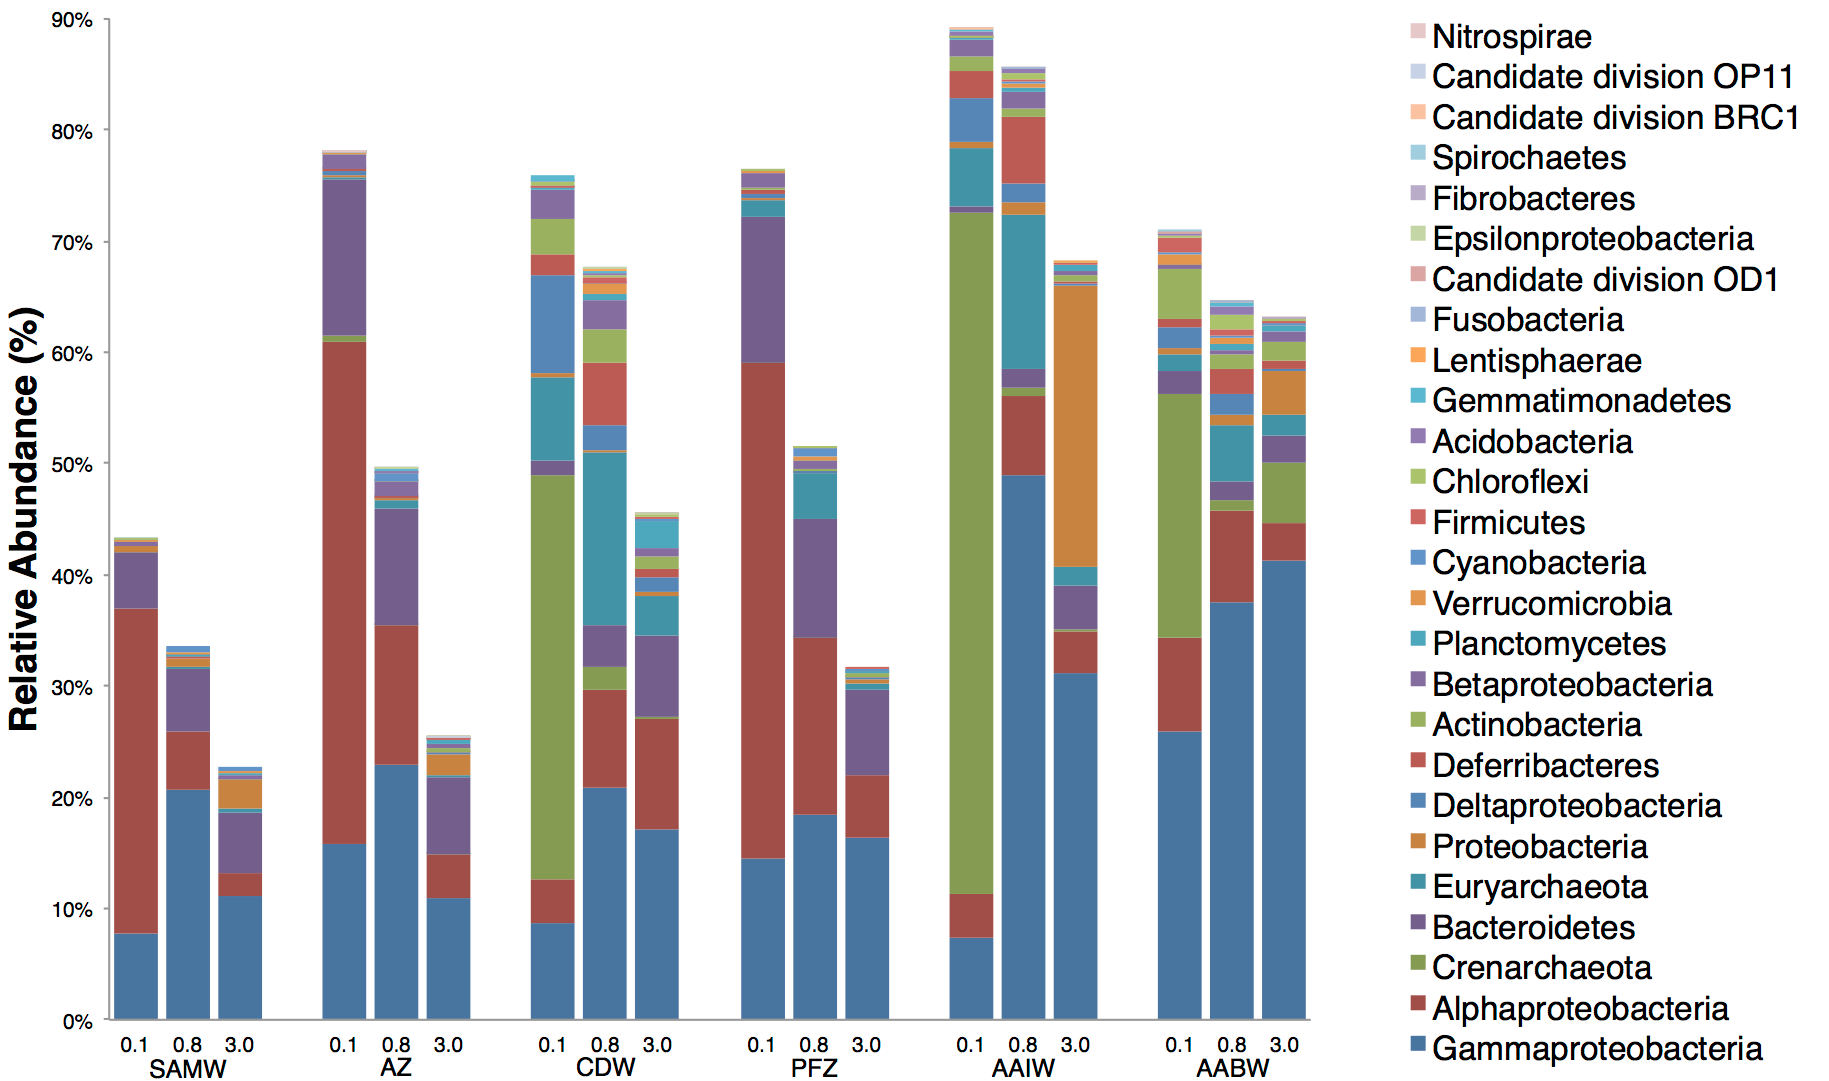
\includegraphics[width=\textwidth]{../advection/taxonomicbarplot.png}
  \caption[OTU assignments in the advection study.]{Taxonomic assignments for each sampled water mass. Water masses (x-axis): Subantarctic Mode Water (SAMW); Antarctic Zone (AZ); Circumpolar Deep Water (CDW); Polar Frontal Zone (PFZ); Antarctic Intermediate Water (AAIW); Antarctic Bottom Water (AABW). Size fractions are given in \micron{}. All \acp{OTU} aggregated to phylum, except for members of the Proteobacteria which were aggregated to class when known. Relative abundance is percentage of all reads assigned to a given taxonomic group and has been scaled to account for unassigned reads.}
  \label{fig:taxonomicbarplot}
\end{figure}
